% ============================================================
% RVT-Swarm: Recoverability-Verified Topological Control
% for Decentralized Swarm Formation
% ============================================================
\documentclass[journal]{IEEEtran}

\usepackage[utf8]{inputenc}
\usepackage[T1]{fontenc}
\usepackage{amsmath,amssymb,amsfonts,bm}
\usepackage{amsthm}
\usepackage{algorithmic}
\usepackage[ruled,vlined,linesnumbered]{algorithm2e}
\makeatletter
\newcommand{\removelatexerror}{\let\@latex@error\@gobble}
\makeatother
\usepackage{graphicx}
\usepackage{float}
\usepackage{booktabs}
\usepackage{multirow}
\usepackage{xcolor}
\usepackage{hyperref}
\usepackage{cleveref}
\usepackage{subcaption}
\usepackage{tikz}
\usetikzlibrary{positioning,arrows.meta,calc,patterns,decorations.pathreplacing}
\usepackage{pifont}
\newcommand{\cmark}{\ding{51}}
\newcommand{\xmark}{\ding{55}}
\newcommand{\pmark}{$\triangle$}

\DeclareMathOperator*{\argmax}{arg\,max}
\DeclareMathOperator*{\argmin}{arg\,min}
\newcommand{\R}{\mathbb{R}}
\newcommand{\cG}{\mathcal{G}}
\newcommand{\cN}{\mathcal{N}}
\newcommand{\cT}{\mathcal{T}}
\newcommand{\cS}{\mathcal{S}}
\newcommand{\bfu}{\mathbf{u}}
\newcommand{\bfp}{\mathbf{p}}
\newcommand{\bfv}{\mathbf{v}}
\newcommand{\bfe}{\mathbf{e}}

\begin{document}

\title{RVT-Swarm: Recoverability-Verified Topological Control\\
for Decentralized Swarm Formation}

\author{Anonymous Authors%
\thanks{Manuscript prepared from the released research prototype codebase.}}

\maketitle

\begin{abstract}
Decentralized swarm formation in cluttered environments requires more
than instantaneous collision avoidance: the team must also preserve the
ability to reorganize and recover a usable formation after passing
through bottlenecks. We present \textbf{RVT-Swarm}, a graph-based
controller that augments per-robot acceleration commands with discrete
topology actions and a learned \emph{recoverability} score map over
candidate formations. Recoverability is defined as a short-horizon
ability to remain collision-free, make goal progress, and return toward
a formation tube under a candidate topology.
RVT-Swarm combines (i) a local interaction-graph encoder with action,
recoverability, uncertainty, and topology heads; (ii) a counterfactual
topology selector with hysteresis and cooldown; and (iii) a lightweight
CBF-inspired progress-preserving projection shield.
Training uses imitation learning plus counterfactual short-horizon
rollouts from a common expert controller. On the current prototype
benchmark (4 scenarios, 4--16 robots), RVT-Swarm reaches the best
composite success rate among all tested methods at \textbf{43.5\%},
compared with \textbf{41.25\%} for InstantCert and \textbf{39.0\%} for
GNN-Only, while also reducing deadlock to \textbf{6.75\%} and
irreversible collapse to \textbf{11.25\%}. The ablation study reveals a
more nuanced picture: the full method improves collision-free execution
and overall benchmark ranking, but some component removals improve
individual metrics, indicating that the current recoverability surrogate
and end-task objective are not yet perfectly aligned. We therefore frame
RVT-Swarm as a strong research scaffold for recoverability-aware swarm
formation control rather than a final benchmark endpoint.
\end{abstract}

\begin{IEEEkeywords}
Multi-robot systems, swarm formation control, graph neural networks,
safety-critical control, topology adaptation, recoverability.
\end{IEEEkeywords}

\section{Introduction}
\label{sec:intro}

Multi-robot formations are useful only when they remain both
\emph{safe} and \emph{task-capable}. In warehouse logistics, cooperative
inspection, or search-and-rescue, a team must not merely avoid
collisions; it must also preserve enough structure to pass through
clutter, regroup, and continue making progress toward a collective
goal~\cite{garg2024safe_multirobot_review,deng2024formation_adaptation,xie2025multi_uav_formation_rl}. This is especially difficult in
decentralized settings with limited local sensing, heterogeneous local
contexts, and team sizes that vary at deployment time.

Existing approaches usually solve only part of this problem.
Graph-based decentralized controllers scale well to large teams but
often optimize local motion directly, without an explicit notion of
whether the team can still \emph{recover} a useful formation after local
reconfiguration~\cite{muthusamy2024gnn_generalizability,goeckner2024magec}.
Control-barrier-function (CBF) approaches provide strong instantaneous
safety structure~\cite{zhang2025gcbf_plus,butler2024collaborative_safety,zhang2025dgppo}, but
they typically reason about collision avoidance rather than return to a
formation tube. Adaptive-formation approaches can change shape to fit
the environment, but usually rely on hand-designed switching logic or
implicit policies without an explicit recoverability score over
alternative topologies~\cite{deng2024formation_adaptation,xie2025multi_uav_formation_rl}.
Reactive methods such as ORCA can maintain goal progress, but often do
so by sacrificing formation quality entirely~\cite{van2011orca}.

This paper explores a different angle: rather than asking only whether
the current action is safe, we ask whether the current local state is
\emph{recoverable} under a small set of candidate formation topologies.
In RVT-Swarm, each local graph observation is mapped not only to a
control action but also to a score map over topological actions
(\textsc{keep}, \textsc{compress}, \textsc{line}, \textsc{split},
\textsc{recover}). The controller then evaluates these topologies
counterfactually and selects the one with the best predicted
recoverability, subject to hysteresis and cooldown. A lightweight
projection-based shield intervenes only when risk is high or when all
candidate topologies appear unrecoverable.

The resulting system is deliberately pragmatic. It does not claim an
exact viability kernel or a formal distributed reachability proof.
Instead, it uses short-horizon counterfactual rollouts to construct a
learned surrogate of recoverability and then deploys that surrogate
online for topology adaptation. This design is consistent with the
current codebase and the current benchmark setting.

\subsection{Contributions}
We make the following contributions:
\begin{enumerate}
    \item We formulate \emph{recoverability-aware topology adaptation}
    for decentralized swarm formation, where candidate formation modes
    are scored by their short-horizon ability to remain safe, make goal
    progress, and return toward a formation tube.

    \item We implement a graph-attention controller with four coupled
    outputs: per-robot accelerations, graph-level topology logits,
    per-topology recoverability scores, and uncertainty estimates. A
    gradient-scaling mechanism reduces interference from auxiliary heads
    on the action pathway.

    \item We introduce a recoverability-aware topology selector with
    hysteresis, cooldown, contextual bonuses, and a progress-preserving
    CBF-inspired projection shield that only activates under elevated
    risk or global negative recoverability.

    \item We provide a unified experimental scaffold with learned
    baselines, historical baselines, rollout-based labels, and liveness
    metrics such as deadlock, topology switching, and irreversible
    collapse. On the current prototype benchmark, RVT-Swarm attains the
    best overall success among tested methods.
\end{enumerate}

\section{Related Work}
\label{sec:related}

\subsection{Decentralized Graph Policies}
Graph neural networks are a natural fit for decentralized multi-robot
control because they preserve permutation invariance and local
communication structure~\cite{muthusamy2024gnn_generalizability,goeckner2024magec}.
Our work follows this line in using a local interaction graph, but adds
explicit topology adaptation and a recoverability score map rather than
predicting control alone.

\subsection{Safety-Critical Multi-Robot Control}
Recent safety-critical multi-robot controllers use graph-structured
certificates, collaborative safety filters, or discrete safe-policy
learning to enforce pairwise constraints in distributed teams~\cite{zhang2025gcbf_plus,butler2024collaborative_safety,zhang2025dgppo}.
Recent graph-CBF work scales safety reasoning through local
graphs~\cite{zhang2025gcbf_plus,zhang2025dgppo}. RVT-Swarm is influenced by this design,
but our shield is intentionally lightweight and approximate: it is a
projection-based correction mechanism rather than a formally certified
QP solver. More importantly, our main decision variable is not only the
continuous action but also the topology under which the swarm remains
recoverable.

\subsection{Adaptive Formation and Recoverability}
Adaptive formation methods change the team geometry to fit corridors,
obstacles, or task context~\cite{deng2024formation_adaptation,xie2025multi_uav_formation_rl}.
Viability and reachability learning study whether a state can remain in
or return to a desirable set over a finite horizon~\cite{abate2024safe_reach_set,
li2025certifiable_reachability,jung2025rail}. RVT-Swarm sits between these directions: it learns a
short-horizon, local-graph surrogate of recoverability and uses it to
guide topology changes. The current implementation should therefore be
understood as a recoverability-informed formation controller rather than
as a formal reachability engine.

To make this positioning explicit, \Cref{tab:comparison} contrasts
RVT-Swarm with representative prior work along the axes that matter most
for the current prototype: local graph execution, formation awareness,
explicit topology adaptation, recoverability modeling, counterfactual
selection, and progress-preserving safety intervention.

\begin{table*}[!t]
\centering
\caption{Positioning of RVT-Swarm relative to representative recent prior work.
\cmark~= primary capability; \pmark~= partially addressed;
\xmark~= not addressed. The table is intended as a qualitative
positioning summary for the current prototype rather than an exhaustive
taxonomy.}
\label{tab:comparison}
\scriptsize
\setlength{\tabcolsep}{4pt}
\renewcommand{\arraystretch}{1.12}
\begin{tabular}{lcc ccccccc}
\toprule
\textbf{Method} & \textbf{Venue} & \textbf{Year}
& \textbf{\shortstack[c]{Local graph\\distributed}}
& \textbf{\shortstack[c]{Formation\\aware}}
& \textbf{\shortstack[c]{Obstacle\\dynamics}}
& \textbf{\shortstack[c]{Topology\\adaptation}}
& \textbf{\shortstack[c]{Recoverability\\model}}
& \textbf{\shortstack[c]{Counterfactual\\selection}}
& \textbf{\shortstack[c]{Progress\\shield}} \\
\midrule
GCBF+~\cite{zhang2025gcbf_plus}
    & T-RO & 2025 & \cmark & \pmark & \cmark
    & \xmark & \xmark & \xmark & \pmark \\
Collab.\ safety form.~\cite{butler2024collaborative_safety}
    & arXiv & 2024 & \cmark & \cmark & \pmark
    & \xmark & \xmark & \xmark & \pmark \\
Neural barrier reach~\cite{abate2024safe_reach_set}
    & IFAC & 2024 & \xmark & \xmark & \pmark
    & \xmark & \cmark & \xmark & \xmark \\
Cert.\ Reach.~\cite{li2025certifiable_reachability}
    & RA-L & 2025 & \pmark & \xmark & \cmark
    & \xmark & \cmark & \xmark & \xmark \\
RAIL~\cite{jung2025rail}
    & ICRA & 2025 & \pmark & \xmark & \cmark
    & \xmark & \cmark & \xmark & \xmark \\
DGPPO~\cite{zhang2025dgppo}
    & ICLR & 2025 & \cmark & \xmark & \cmark
    & \xmark & \xmark & \xmark & \cmark \\
Form.-adapt nav.~\cite{deng2024formation_adaptation}
    & arXiv & 2024 & \cmark & \cmark & \pmark
    & \cmark & \xmark & \xmark & \xmark \\
Multi-UAV RL~\cite{xie2025multi_uav_formation_rl}
    & IROS & 2025 & \cmark & \cmark & \cmark
    & \pmark & \xmark & \xmark & \xmark \\
\midrule
\textbf{RVT-Swarm (ours)}
    & --- & 2026 & \cmark & \cmark & \cmark
    & \cmark & \cmark & \cmark & \cmark \\
\bottomrule
\end{tabular}
\end{table*}

\section{Problem Setup}
\label{sec:problem}

\subsection{Environment and Dynamics}
We consider $N$ robots moving in a 2D workspace with discrete-time
kinematics
\begin{equation}
\bfp_i(t+1) = \bfp_i(t) + \bfv_i(t)\Delta t,\qquad
\bfv_i(t+1) = \bfv_i(t) + \bfu_i(t)\Delta t,
\label{eq:dynamics}
\end{equation}
subject to bounded speed and acceleration.
Each robot observes local relative geometry, obstacle context,
goal direction, formation error, and a 36-ray 270$^\circ$ LiDAR scan.
The environment includes static obstacles, dynamic obstacles, and a
narrow-passage configuration.

\subsection{Formation Tube and Topology Actions}
Let $\bar{\bfp}(t)$ denote the swarm centroid and let
$\{\bm{\delta}_i^\tau\}_{i=1}^N$ denote the desired offsets of topology
$\tau \in \cT$. The current formation error is
\begin{equation}
\bfe_i^\tau(t) = \bar{\bfp}(t) + \bm{\delta}_i^\tau - \bfp_i(t).
\end{equation}
Rather than choosing only a continuous control input, the policy also
selects a discrete \emph{formation mode} (or topology action) from a
small finite set:
\begin{equation}
\cT=\{\textsc{keep},\textsc{compress},\textsc{line},
\textsc{split},\textsc{recover}\}.
\end{equation}
Intuitively, these modes tell the swarm whether to keep its current
shape, compress into a tighter pattern, align into a line, temporarily
split into subgroups, or recover back toward the nominal formation.
These actions control the global formation geometry through scale,
corridor alignment, or temporary splitting/merging.

\subsection{Recoverability}
For a state $s_t$ and topology $\tau$, we define recoverability as a
short-horizon score that rewards collision-free motion, goal progress,
and return toward a formation tube while penalizing deadlock, excessive
switching, and persistent split states:
\begin{equation}
\begin{aligned}
R(s_t;\tau) = \frac{1}{H}\sum_{h=0}^{H-1}
\Bigl[
&w_c c_{t+h} + w_p p_{t+h} + w_f f_{t+h} \\
&- w_d d_{t+h} - w_s q_{t+h}
\Bigr].
\end{aligned}
\label{eq:recoverability}
\end{equation}
Here $c_{t+h}$ is a collision-free indicator, $p_{t+h}$ measures goal
progress, $f_{t+h}$ measures formation-tube recovery, $d_{t+h}$ is a
deadlock-related penalty, and $q_{t+h}$ captures switching/splitting
penalties. In the implementation, these scores are generated by
short-horizon counterfactual rollouts of a common expert controller.

The online objective is then to select $(\bfu,\tau)$ that preserves
progress while favoring positive recoverability:
\begin{equation}
\max_{\bfu,\tau}\;
\alpha\,\text{progress}
\;+\;
\beta\,\text{formation}
\;+\;
\gamma\,\hat{R}(s_t;\tau),
\label{eq:objective}
\end{equation}
where $\hat{R}$ is the learned recoverability surrogate.

\section{Method}
\label{sec:method}

RVT-Swarm combines a graph-attention backbone, a recoverability-aware
multi-head decoder, a counterfactual topology selector, and a
projection-based shield. \Cref{fig:architecture} shows the overall
pipeline and \Cref{fig:rfn} details the recoverability network.

\begin{figure}[H]
\centering
% ============================================================
%  fig_architecture.tex  –  TikZ overview split into training and inference
%  Include via % ============================================================
%  fig_architecture.tex  –  TikZ overview split into training and inference
%  Include via % ============================================================
%  fig_architecture.tex  –  TikZ overview split into training and inference
%  Include via \input{fig_architecture.tex} in main.tex
% ============================================================
\resizebox{\columnwidth}{!}{%
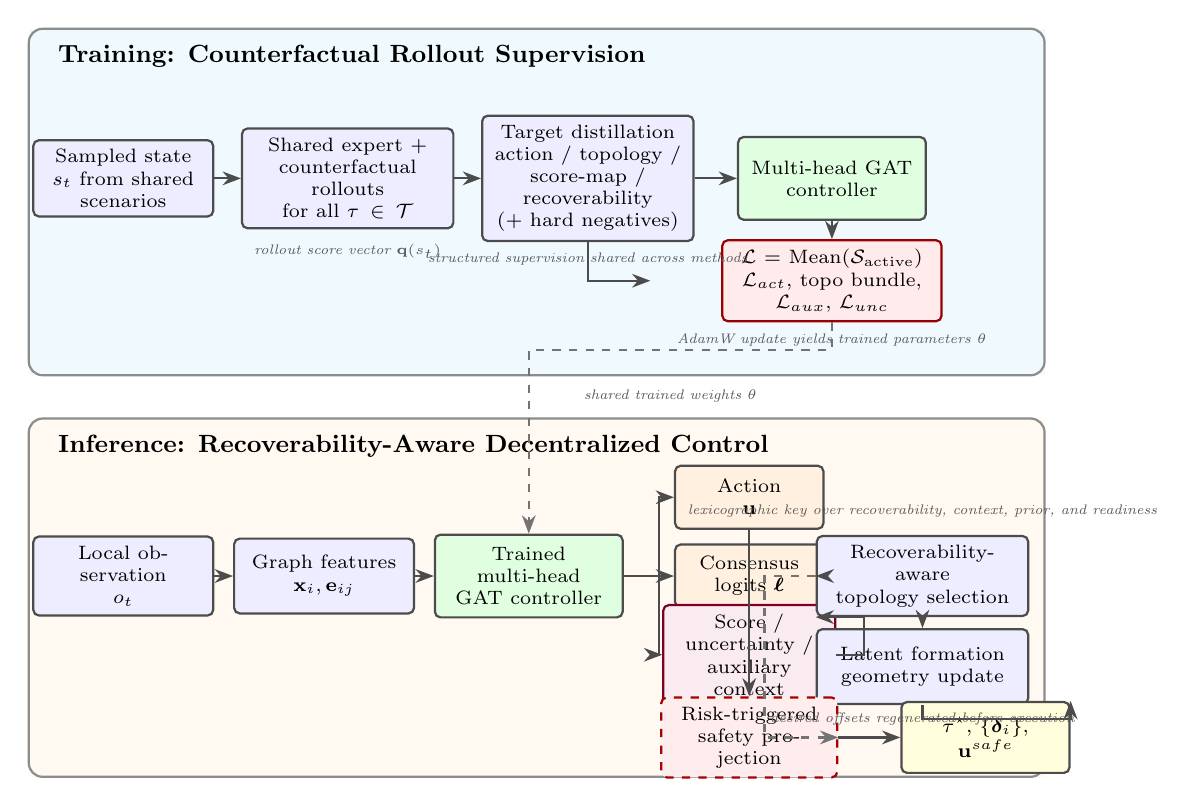
\begin{tikzpicture}[
    >=Stealth,
    arr/.style={->, thick, black!70},
    darr/.style={->, thick, dashed, black!55},
    panel/.style={rounded corners=5pt, draw=black!45, thick},
    title/.style={font=\small\bfseries, anchor=west},
    note/.style={font=\tiny\itshape, text=black!65, align=center},
    box/.style={
        rectangle, rounded corners=2pt, draw=black!70, fill=blue!7,
        minimum height=0.95cm, text width=2.05cm, align=center,
        font=\scriptsize, thick
    },
    wide/.style={
        rectangle, rounded corners=2pt, draw=black!70, fill=blue!7,
        minimum height=0.95cm, text width=2.45cm, align=center,
        font=\scriptsize, thick
    },
    model/.style={
        rectangle, rounded corners=2pt, draw=black!70, fill=green!12,
        minimum height=1.05cm, text width=2.15cm, align=center,
        font=\scriptsize, thick
    },
    loss/.style={
        rectangle, rounded corners=2pt, draw=red!60!black, fill=red!8,
        minimum height=0.95cm, text width=2.55cm, align=center,
        font=\scriptsize, thick
    },
    head/.style={
        rectangle, rounded corners=2pt, draw=black!70, fill=orange!12,
        minimum height=0.8cm, text width=1.65cm, align=center,
        font=\scriptsize, thick
    },
    rec/.style={
        rectangle, rounded corners=2pt, draw=purple!65!black, fill=purple!8,
        minimum height=0.8cm, text width=1.95cm, align=center,
        font=\scriptsize, thick
    },
    shield/.style={
        rectangle, rounded corners=2pt, draw=red!65!black, fill=red!7,
        minimum height=0.8cm, text width=2.0cm, align=center,
        font=\scriptsize, thick, dashed
    },
    final/.style={
        rectangle, rounded corners=2pt, draw=black!70, fill=yellow!14,
        minimum height=0.9cm, text width=1.9cm, align=center,
        font=\scriptsize, thick
    }
]

% ---------------- Panel backgrounds ----------------
\fill[cyan!6] (-0.2,4.55) rectangle (12.7,8.95);
\draw[panel] (-0.2,4.55) rectangle (12.7,8.95);
\node[title] at (0.05,8.6) {Training: Counterfactual Rollout Supervision};

\fill[orange!5] (-0.2,-0.55) rectangle (12.7,4.0);
\draw[panel] (-0.2,-0.55) rectangle (12.7,4.0);
\node[title] at (0.05,3.65) {Inference: Recoverability-Aware Decentralized Control};

% ---------------- Training panel ----------------
\node[box]  (state)   at (1.00,7.05) {Sampled state\\$s_t$ from shared scenarios};
\node[wide] (roll)    at (3.85,7.05) {Shared expert +\\counterfactual rollouts\\for all $\tau \in \mathcal{T}$};
\node[wide] (target)  at (6.90,7.05) {Target distillation\\action / topology /\\score-map / recoverability\\(+ hard negatives)};
\node[model](trainnet)at (10.00,7.05) {Multi-head GAT\\controller};
\node[loss] (loss)    at (10.00,5.75) {$\mathcal{L}=\mathrm{Mean}(\mathcal{S}_{\mathrm{active}})$\\$\mathcal{L}_{act}$, topo bundle,\\$\mathcal{L}_{aux}$, $\mathcal{L}_{unc}$};

\draw[arr] (state.east) -- (roll.west);
\draw[arr] (roll.east) -- (target.west);
\draw[arr] (target.east) -- (trainnet.west);
\draw[arr] (trainnet.south) -- (loss.north);
\draw[arr] (target.south) |- ([xshift=-0.9cm]loss.west);

\node[note] at (3.85,6.12) {rollout score vector $\mathbf{q}(s_t)$};
\node[note] at (6.90,6.02) {structured supervision shared across methods};
\node[note] at (10.00,5.00) {AdamW update yields trained parameters $\theta$};

% ---------------- Inference panel ----------------
\node[box]   (obs)     at (1.00,2.00) {Local observation\\$o_t$};
\node[box]   (graph)   at (3.55,2.00) {Graph features\\$\mathbf{x}_i,\mathbf{e}_{ij}$};
\node[model] (infnet)  at (6.15,2.00) {Trained multi-head\\GAT controller};
\node[head]  (act)     at (8.95,3.00) {Action\\$\bfu$};
\node[head]  (logit)   at (8.95,2.00) {Consensus\\logits $\bm{\ell}$};
\node[rec]   (score)   at (8.95,1.00) {Score / uncertainty /\\auxiliary context};
\node[wide]  (select)  at (11.15,2.00) {Recoverability-aware\\topology selection};
\node[wide]  (geom)    at (11.15,0.85) {Latent formation\\geometry update};
\node[shield](shield)  at (8.95,-0.05) {Risk-triggered\\safety projection};
\node[final] (out)     at (11.95,-0.05) {$\tau^\star$, $\{\bm{\delta}_i\}$,\\$\bfu^{safe}$};

\draw[arr] (obs.east) -- (graph.west);
\draw[arr] (graph.east) -- (infnet.west);
\draw[arr] (infnet.east) -- ++(0.45,0) |- (act.west);
\draw[arr] (infnet.east) -- (logit.west);
\draw[arr] (infnet.east) -- ++(0.45,0) |- (score.west);
\draw[arr] (logit.east) -- (select.west);
\draw[arr] (score.east) -- ++(0.35,0) |- (select.south west);
\draw[arr] (select.south) -- (geom.north);
\draw[arr] (act.south) -- (shield.north);
\draw[darr] (select.west) -- ++(-0.65,0) |- (shield.east);
\draw[arr] (geom.south) -- ++(0,-0.18) -| (out.north east);
\draw[arr] (shield.east) -- (out.west);

\draw[darr] (loss.south) -- ++(0,-0.35) -| (infnet.north);
\node[note] at (7.95,4.28) {shared trained weights $\theta$};
\node[note] at (11.15,2.83) {lexicographic key over recoverability, context, prior, and readiness};
\node[note] at (11.15,0.18) {desired offsets regenerated before execution};

\end{tikzpicture}%
}
 in main.tex
% ============================================================
\resizebox{\columnwidth}{!}{%
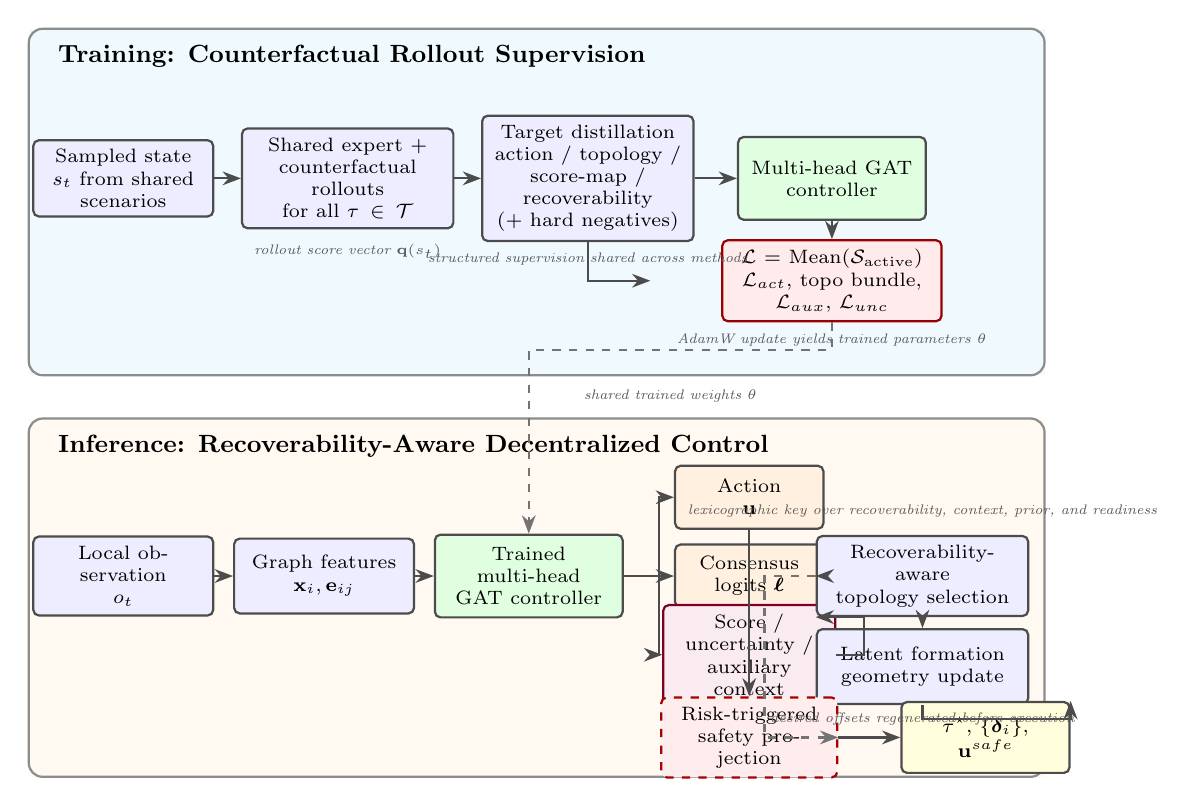
\begin{tikzpicture}[
    >=Stealth,
    arr/.style={->, thick, black!70},
    darr/.style={->, thick, dashed, black!55},
    panel/.style={rounded corners=5pt, draw=black!45, thick},
    title/.style={font=\small\bfseries, anchor=west},
    note/.style={font=\tiny\itshape, text=black!65, align=center},
    box/.style={
        rectangle, rounded corners=2pt, draw=black!70, fill=blue!7,
        minimum height=0.95cm, text width=2.05cm, align=center,
        font=\scriptsize, thick
    },
    wide/.style={
        rectangle, rounded corners=2pt, draw=black!70, fill=blue!7,
        minimum height=0.95cm, text width=2.45cm, align=center,
        font=\scriptsize, thick
    },
    model/.style={
        rectangle, rounded corners=2pt, draw=black!70, fill=green!12,
        minimum height=1.05cm, text width=2.15cm, align=center,
        font=\scriptsize, thick
    },
    loss/.style={
        rectangle, rounded corners=2pt, draw=red!60!black, fill=red!8,
        minimum height=0.95cm, text width=2.55cm, align=center,
        font=\scriptsize, thick
    },
    head/.style={
        rectangle, rounded corners=2pt, draw=black!70, fill=orange!12,
        minimum height=0.8cm, text width=1.65cm, align=center,
        font=\scriptsize, thick
    },
    rec/.style={
        rectangle, rounded corners=2pt, draw=purple!65!black, fill=purple!8,
        minimum height=0.8cm, text width=1.95cm, align=center,
        font=\scriptsize, thick
    },
    shield/.style={
        rectangle, rounded corners=2pt, draw=red!65!black, fill=red!7,
        minimum height=0.8cm, text width=2.0cm, align=center,
        font=\scriptsize, thick, dashed
    },
    final/.style={
        rectangle, rounded corners=2pt, draw=black!70, fill=yellow!14,
        minimum height=0.9cm, text width=1.9cm, align=center,
        font=\scriptsize, thick
    }
]

% ---------------- Panel backgrounds ----------------
\fill[cyan!6] (-0.2,4.55) rectangle (12.7,8.95);
\draw[panel] (-0.2,4.55) rectangle (12.7,8.95);
\node[title] at (0.05,8.6) {Training: Counterfactual Rollout Supervision};

\fill[orange!5] (-0.2,-0.55) rectangle (12.7,4.0);
\draw[panel] (-0.2,-0.55) rectangle (12.7,4.0);
\node[title] at (0.05,3.65) {Inference: Recoverability-Aware Decentralized Control};

% ---------------- Training panel ----------------
\node[box]  (state)   at (1.00,7.05) {Sampled state\\$s_t$ from shared scenarios};
\node[wide] (roll)    at (3.85,7.05) {Shared expert +\\counterfactual rollouts\\for all $\tau \in \mathcal{T}$};
\node[wide] (target)  at (6.90,7.05) {Target distillation\\action / topology /\\score-map / recoverability\\(+ hard negatives)};
\node[model](trainnet)at (10.00,7.05) {Multi-head GAT\\controller};
\node[loss] (loss)    at (10.00,5.75) {$\mathcal{L}=\mathrm{Mean}(\mathcal{S}_{\mathrm{active}})$\\$\mathcal{L}_{act}$, topo bundle,\\$\mathcal{L}_{aux}$, $\mathcal{L}_{unc}$};

\draw[arr] (state.east) -- (roll.west);
\draw[arr] (roll.east) -- (target.west);
\draw[arr] (target.east) -- (trainnet.west);
\draw[arr] (trainnet.south) -- (loss.north);
\draw[arr] (target.south) |- ([xshift=-0.9cm]loss.west);

\node[note] at (3.85,6.12) {rollout score vector $\mathbf{q}(s_t)$};
\node[note] at (6.90,6.02) {structured supervision shared across methods};
\node[note] at (10.00,5.00) {AdamW update yields trained parameters $\theta$};

% ---------------- Inference panel ----------------
\node[box]   (obs)     at (1.00,2.00) {Local observation\\$o_t$};
\node[box]   (graph)   at (3.55,2.00) {Graph features\\$\mathbf{x}_i,\mathbf{e}_{ij}$};
\node[model] (infnet)  at (6.15,2.00) {Trained multi-head\\GAT controller};
\node[head]  (act)     at (8.95,3.00) {Action\\$\bfu$};
\node[head]  (logit)   at (8.95,2.00) {Consensus\\logits $\bm{\ell}$};
\node[rec]   (score)   at (8.95,1.00) {Score / uncertainty /\\auxiliary context};
\node[wide]  (select)  at (11.15,2.00) {Recoverability-aware\\topology selection};
\node[wide]  (geom)    at (11.15,0.85) {Latent formation\\geometry update};
\node[shield](shield)  at (8.95,-0.05) {Risk-triggered\\safety projection};
\node[final] (out)     at (11.95,-0.05) {$\tau^\star$, $\{\bm{\delta}_i\}$,\\$\bfu^{safe}$};

\draw[arr] (obs.east) -- (graph.west);
\draw[arr] (graph.east) -- (infnet.west);
\draw[arr] (infnet.east) -- ++(0.45,0) |- (act.west);
\draw[arr] (infnet.east) -- (logit.west);
\draw[arr] (infnet.east) -- ++(0.45,0) |- (score.west);
\draw[arr] (logit.east) -- (select.west);
\draw[arr] (score.east) -- ++(0.35,0) |- (select.south west);
\draw[arr] (select.south) -- (geom.north);
\draw[arr] (act.south) -- (shield.north);
\draw[darr] (select.west) -- ++(-0.65,0) |- (shield.east);
\draw[arr] (geom.south) -- ++(0,-0.18) -| (out.north east);
\draw[arr] (shield.east) -- (out.west);

\draw[darr] (loss.south) -- ++(0,-0.35) -| (infnet.north);
\node[note] at (7.95,4.28) {shared trained weights $\theta$};
\node[note] at (11.15,2.83) {lexicographic key over recoverability, context, prior, and readiness};
\node[note] at (11.15,0.18) {desired offsets regenerated before execution};

\end{tikzpicture}%
}
 in main.tex
% ============================================================
\resizebox{\columnwidth}{!}{%
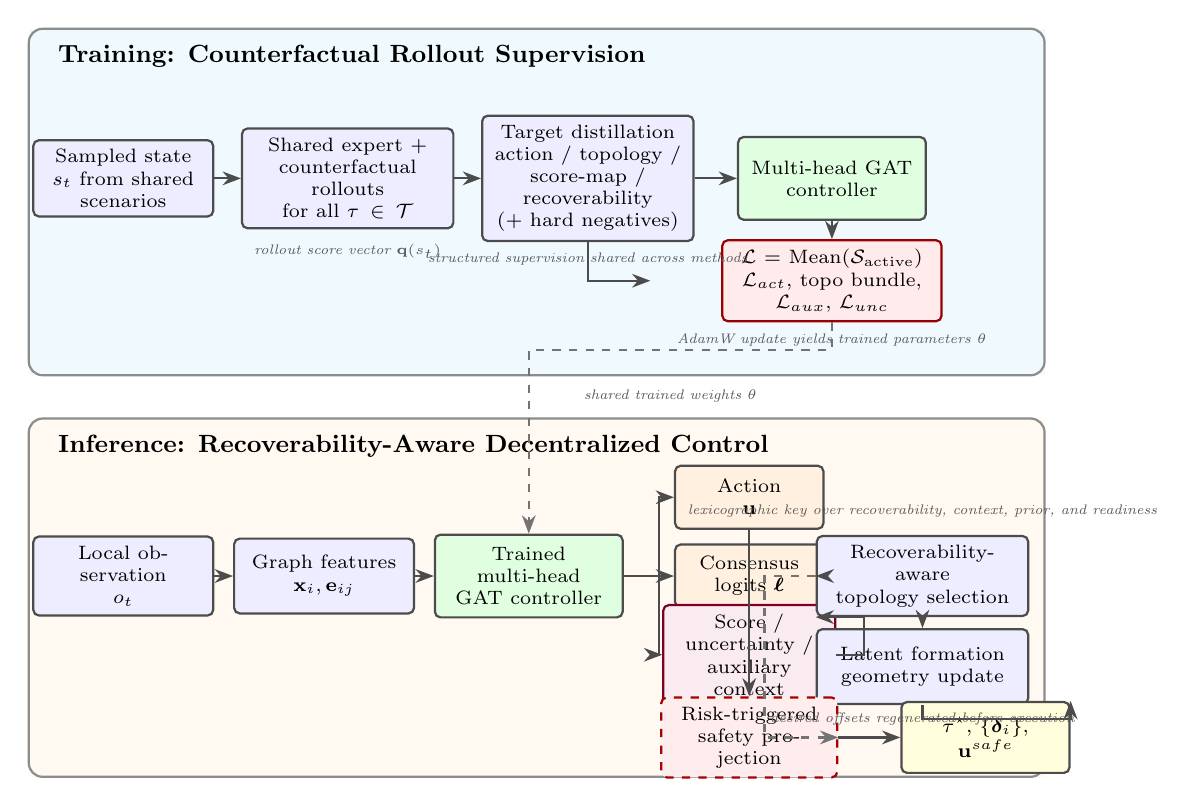
\begin{tikzpicture}[
    >=Stealth,
    arr/.style={->, thick, black!70},
    darr/.style={->, thick, dashed, black!55},
    panel/.style={rounded corners=5pt, draw=black!45, thick},
    title/.style={font=\small\bfseries, anchor=west},
    note/.style={font=\tiny\itshape, text=black!65, align=center},
    box/.style={
        rectangle, rounded corners=2pt, draw=black!70, fill=blue!7,
        minimum height=0.95cm, text width=2.05cm, align=center,
        font=\scriptsize, thick
    },
    wide/.style={
        rectangle, rounded corners=2pt, draw=black!70, fill=blue!7,
        minimum height=0.95cm, text width=2.45cm, align=center,
        font=\scriptsize, thick
    },
    model/.style={
        rectangle, rounded corners=2pt, draw=black!70, fill=green!12,
        minimum height=1.05cm, text width=2.15cm, align=center,
        font=\scriptsize, thick
    },
    loss/.style={
        rectangle, rounded corners=2pt, draw=red!60!black, fill=red!8,
        minimum height=0.95cm, text width=2.55cm, align=center,
        font=\scriptsize, thick
    },
    head/.style={
        rectangle, rounded corners=2pt, draw=black!70, fill=orange!12,
        minimum height=0.8cm, text width=1.65cm, align=center,
        font=\scriptsize, thick
    },
    rec/.style={
        rectangle, rounded corners=2pt, draw=purple!65!black, fill=purple!8,
        minimum height=0.8cm, text width=1.95cm, align=center,
        font=\scriptsize, thick
    },
    shield/.style={
        rectangle, rounded corners=2pt, draw=red!65!black, fill=red!7,
        minimum height=0.8cm, text width=2.0cm, align=center,
        font=\scriptsize, thick, dashed
    },
    final/.style={
        rectangle, rounded corners=2pt, draw=black!70, fill=yellow!14,
        minimum height=0.9cm, text width=1.9cm, align=center,
        font=\scriptsize, thick
    }
]

% ---------------- Panel backgrounds ----------------
\fill[cyan!6] (-0.2,4.55) rectangle (12.7,8.95);
\draw[panel] (-0.2,4.55) rectangle (12.7,8.95);
\node[title] at (0.05,8.6) {Training: Counterfactual Rollout Supervision};

\fill[orange!5] (-0.2,-0.55) rectangle (12.7,4.0);
\draw[panel] (-0.2,-0.55) rectangle (12.7,4.0);
\node[title] at (0.05,3.65) {Inference: Recoverability-Aware Decentralized Control};

% ---------------- Training panel ----------------
\node[box]  (state)   at (1.00,7.05) {Sampled state\\$s_t$ from shared scenarios};
\node[wide] (roll)    at (3.85,7.05) {Shared expert +\\counterfactual rollouts\\for all $\tau \in \mathcal{T}$};
\node[wide] (target)  at (6.90,7.05) {Target distillation\\action / topology /\\score-map / recoverability\\(+ hard negatives)};
\node[model](trainnet)at (10.00,7.05) {Multi-head GAT\\controller};
\node[loss] (loss)    at (10.00,5.75) {$\mathcal{L}=\mathrm{Mean}(\mathcal{S}_{\mathrm{active}})$\\$\mathcal{L}_{act}$, topo bundle,\\$\mathcal{L}_{aux}$, $\mathcal{L}_{unc}$};

\draw[arr] (state.east) -- (roll.west);
\draw[arr] (roll.east) -- (target.west);
\draw[arr] (target.east) -- (trainnet.west);
\draw[arr] (trainnet.south) -- (loss.north);
\draw[arr] (target.south) |- ([xshift=-0.9cm]loss.west);

\node[note] at (3.85,6.12) {rollout score vector $\mathbf{q}(s_t)$};
\node[note] at (6.90,6.02) {structured supervision shared across methods};
\node[note] at (10.00,5.00) {AdamW update yields trained parameters $\theta$};

% ---------------- Inference panel ----------------
\node[box]   (obs)     at (1.00,2.00) {Local observation\\$o_t$};
\node[box]   (graph)   at (3.55,2.00) {Graph features\\$\mathbf{x}_i,\mathbf{e}_{ij}$};
\node[model] (infnet)  at (6.15,2.00) {Trained multi-head\\GAT controller};
\node[head]  (act)     at (8.95,3.00) {Action\\$\bfu$};
\node[head]  (logit)   at (8.95,2.00) {Consensus\\logits $\bm{\ell}$};
\node[rec]   (score)   at (8.95,1.00) {Score / uncertainty /\\auxiliary context};
\node[wide]  (select)  at (11.15,2.00) {Recoverability-aware\\topology selection};
\node[wide]  (geom)    at (11.15,0.85) {Latent formation\\geometry update};
\node[shield](shield)  at (8.95,-0.05) {Risk-triggered\\safety projection};
\node[final] (out)     at (11.95,-0.05) {$\tau^\star$, $\{\bm{\delta}_i\}$,\\$\bfu^{safe}$};

\draw[arr] (obs.east) -- (graph.west);
\draw[arr] (graph.east) -- (infnet.west);
\draw[arr] (infnet.east) -- ++(0.45,0) |- (act.west);
\draw[arr] (infnet.east) -- (logit.west);
\draw[arr] (infnet.east) -- ++(0.45,0) |- (score.west);
\draw[arr] (logit.east) -- (select.west);
\draw[arr] (score.east) -- ++(0.35,0) |- (select.south west);
\draw[arr] (select.south) -- (geom.north);
\draw[arr] (act.south) -- (shield.north);
\draw[darr] (select.west) -- ++(-0.65,0) |- (shield.east);
\draw[arr] (geom.south) -- ++(0,-0.18) -| (out.north east);
\draw[arr] (shield.east) -- (out.west);

\draw[darr] (loss.south) -- ++(0,-0.35) -| (infnet.north);
\node[note] at (7.95,4.28) {shared trained weights $\theta$};
\node[note] at (11.15,2.83) {lexicographic key over recoverability, context, prior, and readiness};
\node[note] at (11.15,0.18) {desired offsets regenerated before execution};

\end{tikzpicture}%
}

\caption{Overview of RVT-Swarm. Local graph observations feed a shared
graph-attention encoder whose outputs are decoded into control actions,
topology logits, and per-topology recoverability scores. A
counterfactual selector and a lightweight projection shield operate only
at inference time.}
\label{fig:architecture}
\end{figure}

\subsection{Local Graph Encoder}
\label{sec:encoder}

At each step, the swarm builds a $k$-nearest-neighbor interaction graph
with $k=6$. Each node contains a 68-dimensional feature vector
including position, velocity, heading, goal vector, centroid-relative
position, formation error, obstacle-relative cues, topology encoding,
normalized minimum TTC proxy, and 36 normalized LiDAR ranges. Each edge
contains 11-dimensional relational features, including relative
position, relative velocity, spacing error, corridor projections, and a
TTC-style safety descriptor.

The graph is processed by three attention-weighted message-passing
layers. For edge $(j \rightarrow i)$, an edge MLP produces a message
$\mathbf{m}_{ij}$ and a learned attention weight $\alpha_{ij}$, and the
node update is
\begin{align}
\mathbf{m}_{ij} &= \phi_e([\mathbf{h}_i \| \mathbf{h}_j \|
\mathbf{e}_{ij}]), \\
\alpha_{ij} &= \operatorname{softmax}_{j \in \cN(i)}
\bigl(\phi_a(\mathbf{m}_{ij})\bigr), \\
\mathbf{h}_i' &= \mathbf{h}_i +
\phi_n\Bigl(\bigl[\mathbf{h}_i \;\|\;
\sum_{j\in\cN(i)}\alpha_{ij}\mathbf{m}_{ij}\bigr]\Bigr).
\end{align}
The hidden dimension is 128 throughout.

\subsection{Recoverability Field Network}
\label{sec:rfn}

The shared backbone feeds four decoders:
\begin{itemize}
    \item an \textbf{action head} producing per-robot accelerations
    $\bfu_i \in \R^2$;
    \item a \textbf{topology consensus head} producing graph-level
    logits over $\cT$;
    \item a \textbf{score head} producing per-topology recoverability
    scores;
    \item an \textbf{uncertainty head} producing a nonnegative
    uncertainty estimate for each candidate topology.
\end{itemize}

The topology head is not a simple pooled classifier. Each node first
casts a topology vote, neighbor votes are aggregated into mean and
spread statistics, and a small agreement MLP refines these votes before
graph-level pooling. This gives the model a limited form of local
consensus without requiring explicit communication optimization. The
consensus path is summarized in \Cref{alg:consensus}.

\removelatexerror
\begin{algorithm}[H]
\caption{Neighborhood Topology Consensus}
\label{alg:consensus}
\SetAlgoLined
\KwIn{Node embeddings $\{\mathbf{h}_i\}$ and graph neighborhood $\cN(i)$}
\KwOut{Graph-level topology logits $\bm{\ell}$}
$\mathbf{v}_i \leftarrow \mathrm{MLP}_{\mathrm{vote}}(\mathbf{h}_i)$
\quad $\forall i$\;
$\bar{\mathbf{v}}_i \leftarrow \mathrm{MeanAgg}_{j\in \cN(i)}(\mathbf{v}_j)$\;
$\bm{\sigma}_i \leftarrow \sqrt{\mathrm{VarAgg}_{j\in \cN(i)}(\mathbf{v}_j)+\epsilon}$\;
$\hat{\mathbf{v}}_i \leftarrow \mathrm{MLP}_{\mathrm{agree}}
\bigl([\mathbf{v}_i \| \bar{\mathbf{v}}_i \| \bm{\sigma}_i]\bigr)$\;
$\bm{\ell} \leftarrow \mathrm{MeanPool}(\hat{\mathbf{v}}_i)$\;
\Return{$\bm{\ell}$}
\end{algorithm}

Recoverability scores are adjusted by uncertainty:
\begin{equation}
\tilde{r}_\tau = \hat{r}_\tau - 0.25\,\hat{\sigma}_{\tau},\qquad
\hat{R}(s_t) = \max_{\tau \in \cT} \tilde{r}_\tau .
\label{eq:adjusted_recover}
\end{equation}
Only the action head receives full-strength gradients from the backbone.
Before feeding the auxiliary heads, we apply gradient scaling with
factor $0.2$ to reduce degradation of control quality under multitask
training.

\begin{figure*}[!t]
\centering
% ============================================================
%  fig_rfn.tex  –  TikZ: Recoverability Field Network detail
%  Include via % ============================================================
%  fig_rfn.tex  –  TikZ: Recoverability Field Network detail
%  Include via % ============================================================
%  fig_rfn.tex  –  TikZ: Recoverability Field Network detail
%  Include via \input{fig_rfn.tex} in main.tex
% ============================================================
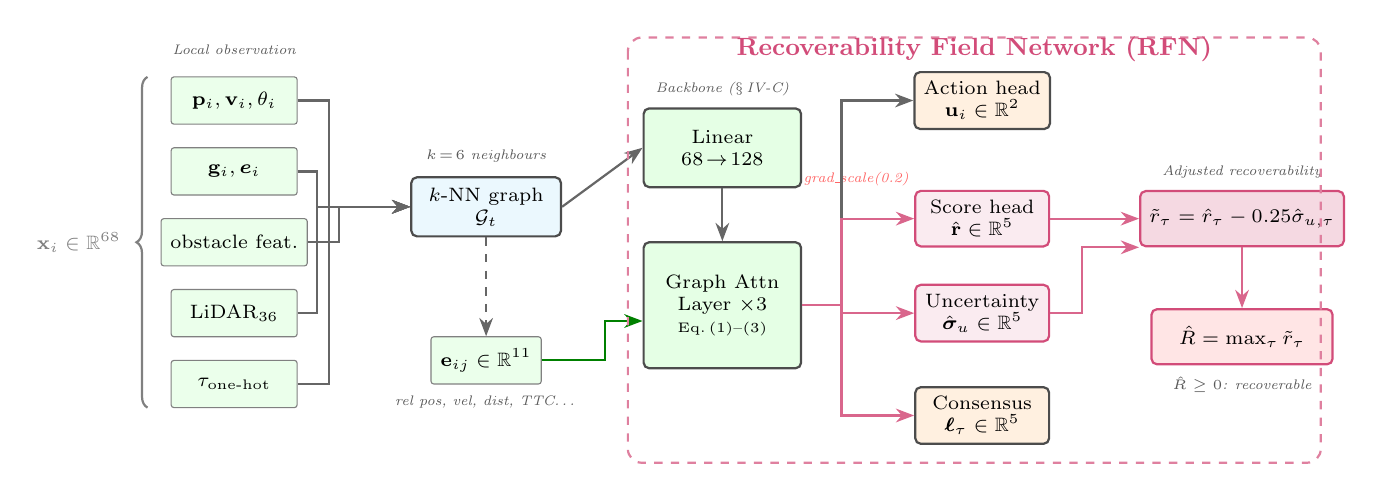
\begin{tikzpicture}[
    >=Stealth,
    block/.style={
        rectangle, draw=black!70, fill=blue!6,
        minimum height=0.75cm, minimum width=1.9cm,
        font=\scriptsize, align=center, rounded corners=2pt,
        thick
    },
    feat/.style={
        rectangle, draw=black!50, fill=green!8,
        minimum height=0.6cm, minimum width=1.6cm,
        font=\scriptsize, align=center, rounded corners=1pt,
    },
    head/.style={
        rectangle, draw=black!70, fill=orange!12,
        minimum height=0.7cm, minimum width=1.7cm,
        font=\scriptsize, align=center, rounded corners=2pt,
        thick
    },
    score/.style={
        rectangle, draw=purple!70, fill=purple!8,
        minimum height=0.7cm, minimum width=1.7cm,
        font=\scriptsize, align=center, rounded corners=2pt,
        thick
    },
    arr/.style={->, thick, black!60},
    garr/.style={->, thick, green!50!black},
    parr/.style={->, thick, purple!60},
    note/.style={font=\tiny\itshape, text=gray!70!black},
]

% ── Column 1: Observation ──
\node[feat] (pos)   at (0, 0.0) {$\bfp_i, \bfv_i, \theta_i$};
\node[feat] (goal)  at (0,-0.9) {$\mathbf{g}_i, \bm{e}_i$};
\node[feat] (obs)   at (0,-1.8) {obstacle feat.};
\node[feat] (lidar) at (0,-2.7) {LiDAR$_{36}$};
\node[feat] (topo)  at (0,-3.6) {$\tau_{\text{one-hot}}$};

\node[note, above=0.15cm of pos] {Local observation};

% ── Brace ──
\draw[decorate, decoration={brace, amplitude=4pt, mirror},
      thick, black!50]
    (-1.1, 0.3) -- (-1.1,-3.9)
    node[midway, left=6pt, font=\scriptsize, align=right]
    {$\mathbf{x}_i \in \mathbb{R}^{68}$};

% ── Column 2: Graph construction ──
\node[block, fill=cyan!8] (knn) at (3.2,-1.35)
    {$k$-NN graph\\$\mathcal{G}_t$};
\node[note, above=0.05cm of knn] {$k\!=\!6$ neighbours};

\draw[arr] (pos.east)   -- ++(0.4,0) |- (knn.west);
\draw[arr] (goal.east)  -- ++(0.25,0) |- (knn.west);
\draw[arr] (obs.east)   -- ++(0.4,0) |- (knn.west);
\draw[arr] (lidar.east) -- ++(0.25,0) |- (knn.west);
\draw[arr] (topo.east)  -- ++(0.4,0) |- (knn.west);

% ── Edge features label ──
\node[feat, minimum width=1.4cm] (efeat) at (3.2,-3.3)
    {$\mathbf{e}_{ij} \in \mathbb{R}^{11}$};
\node[note, below=0.02cm of efeat]
    {rel pos, vel, dist, TTC\ldots};
\draw[arr, dashed] (knn.south) -- (efeat.north);

% ── Column 3: Backbone ──
\node[block, fill=green!10, minimum height=1.0cm,
      minimum width=2.0cm]
    (enc) at (6.2,-0.6) {Linear\\$68 \!\to\! 128$};
\node[block, fill=green!10, minimum height=1.6cm,
      minimum width=2.0cm]
    (gat) at (6.2,-2.6) {Graph Attn\\Layer $\times 3$\\{\tiny Eq.\,(1)--(3)}};

\draw[arr] (knn.east) -- (enc.west);
\draw[arr] (enc.south) -- (gat.north);
\draw[garr] (efeat.east) -- ++(0.8,0) |- ([yshift=-0.2cm]gat.west);

\node[note] at (6.2, 0.15) {Backbone ($\S$\,IV-C)};

% ── Column 4: Heads (branch) ──
% Action
\node[head] (act) at (9.5, 0.0)
    {Action head\\$\bfu_i \in \mathbb{R}^2$};
% Score
\node[score] (rscore) at (9.5,-1.5)
    {Score head\\$\hat{\mathbf{r}} \in \mathbb{R}^5$};
% Uncertainty
\node[score] (unc) at (9.5,-2.7)
    {Uncertainty\\$\hat{\bm{\sigma}}_u \in \mathbb{R}^5$};
% Consensus
\node[head] (cons) at (9.5,-4.0)
    {Consensus\\$\bm{\ell}_\tau \in \mathbb{R}^5$};

% grad scale annotation
\node[note] at (7.9, -1.0) {\textcolor{red!60}{grad\_scale(0.2)}};

\draw[arr] (gat.east) -- ++(0.5,0) |- (act.west);
\draw[parr] (gat.east) -- ++(0.5,0) |- (rscore.west);
\draw[parr] (gat.east) -- ++(0.5,0) |- (unc.west);
\draw[parr] (gat.east) -- ++(0.5,0) |- (cons.west);

% ── Column 5: RFN output ──
\node[score, fill=purple!15, minimum width=2.3cm]
    (rfn_out) at (12.8,-1.5)
    {$\tilde{r}_\tau = \hat{r}_\tau - 0.25\hat{\sigma}_{u,\tau}$};
\node[note, above=0.02cm of rfn_out]
    {Adjusted recoverability};
\draw[parr] (rscore.east) -- (rfn_out.west);
\draw[parr] (unc.east) -- ++(0.4,0) |- (rfn_out.south west);

% RFN margin
\node[score, fill=red!10, minimum width=2.3cm]
    (margin) at (12.8,-3.0)
    {$\hat{R} = \max_\tau \tilde{r}_\tau$};
\draw[parr] (rfn_out.south) -- (margin.north);

\node[note, below=0.02cm of margin]
    {$\hat{R} \ge 0$: recoverable};

% ── Dashed box: RFN ──
\draw[thick, dashed, purple!50, rounded corners=5pt]
    (5.0, 0.8) rectangle (13.8, -4.6);
\node[font=\small\bfseries, text=purple!70]
    at (9.4, 0.65) {Recoverability Field Network (RFN)};

\end{tikzpicture}
 in main.tex
% ============================================================
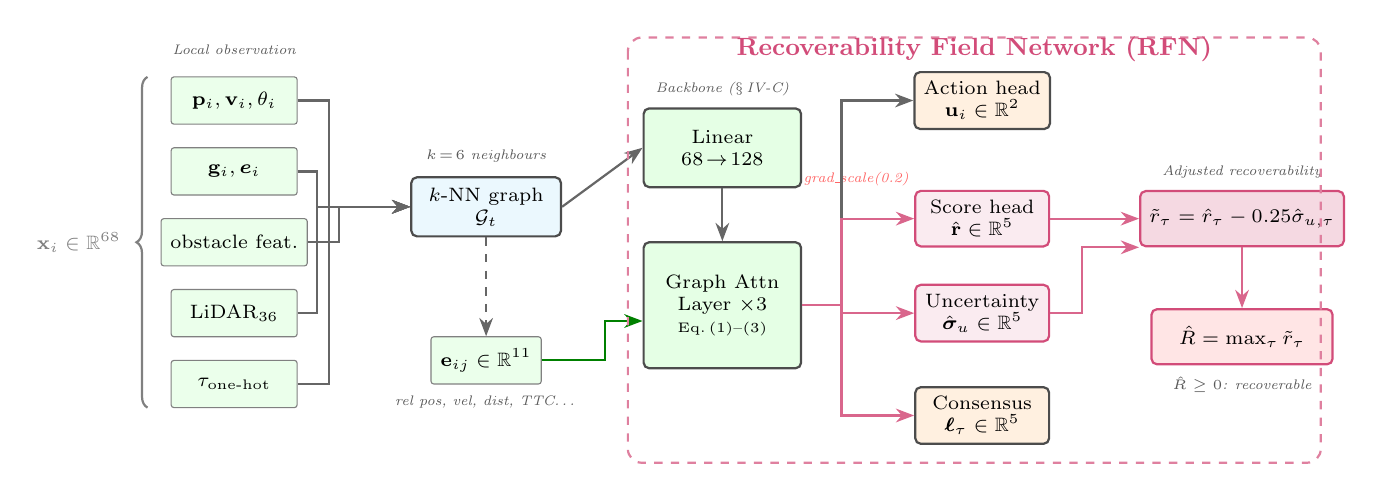
\begin{tikzpicture}[
    >=Stealth,
    block/.style={
        rectangle, draw=black!70, fill=blue!6,
        minimum height=0.75cm, minimum width=1.9cm,
        font=\scriptsize, align=center, rounded corners=2pt,
        thick
    },
    feat/.style={
        rectangle, draw=black!50, fill=green!8,
        minimum height=0.6cm, minimum width=1.6cm,
        font=\scriptsize, align=center, rounded corners=1pt,
    },
    head/.style={
        rectangle, draw=black!70, fill=orange!12,
        minimum height=0.7cm, minimum width=1.7cm,
        font=\scriptsize, align=center, rounded corners=2pt,
        thick
    },
    score/.style={
        rectangle, draw=purple!70, fill=purple!8,
        minimum height=0.7cm, minimum width=1.7cm,
        font=\scriptsize, align=center, rounded corners=2pt,
        thick
    },
    arr/.style={->, thick, black!60},
    garr/.style={->, thick, green!50!black},
    parr/.style={->, thick, purple!60},
    note/.style={font=\tiny\itshape, text=gray!70!black},
]

% ── Column 1: Observation ──
\node[feat] (pos)   at (0, 0.0) {$\bfp_i, \bfv_i, \theta_i$};
\node[feat] (goal)  at (0,-0.9) {$\mathbf{g}_i, \bm{e}_i$};
\node[feat] (obs)   at (0,-1.8) {obstacle feat.};
\node[feat] (lidar) at (0,-2.7) {LiDAR$_{36}$};
\node[feat] (topo)  at (0,-3.6) {$\tau_{\text{one-hot}}$};

\node[note, above=0.15cm of pos] {Local observation};

% ── Brace ──
\draw[decorate, decoration={brace, amplitude=4pt, mirror},
      thick, black!50]
    (-1.1, 0.3) -- (-1.1,-3.9)
    node[midway, left=6pt, font=\scriptsize, align=right]
    {$\mathbf{x}_i \in \mathbb{R}^{68}$};

% ── Column 2: Graph construction ──
\node[block, fill=cyan!8] (knn) at (3.2,-1.35)
    {$k$-NN graph\\$\mathcal{G}_t$};
\node[note, above=0.05cm of knn] {$k\!=\!6$ neighbours};

\draw[arr] (pos.east)   -- ++(0.4,0) |- (knn.west);
\draw[arr] (goal.east)  -- ++(0.25,0) |- (knn.west);
\draw[arr] (obs.east)   -- ++(0.4,0) |- (knn.west);
\draw[arr] (lidar.east) -- ++(0.25,0) |- (knn.west);
\draw[arr] (topo.east)  -- ++(0.4,0) |- (knn.west);

% ── Edge features label ──
\node[feat, minimum width=1.4cm] (efeat) at (3.2,-3.3)
    {$\mathbf{e}_{ij} \in \mathbb{R}^{11}$};
\node[note, below=0.02cm of efeat]
    {rel pos, vel, dist, TTC\ldots};
\draw[arr, dashed] (knn.south) -- (efeat.north);

% ── Column 3: Backbone ──
\node[block, fill=green!10, minimum height=1.0cm,
      minimum width=2.0cm]
    (enc) at (6.2,-0.6) {Linear\\$68 \!\to\! 128$};
\node[block, fill=green!10, minimum height=1.6cm,
      minimum width=2.0cm]
    (gat) at (6.2,-2.6) {Graph Attn\\Layer $\times 3$\\{\tiny Eq.\,(1)--(3)}};

\draw[arr] (knn.east) -- (enc.west);
\draw[arr] (enc.south) -- (gat.north);
\draw[garr] (efeat.east) -- ++(0.8,0) |- ([yshift=-0.2cm]gat.west);

\node[note] at (6.2, 0.15) {Backbone ($\S$\,IV-C)};

% ── Column 4: Heads (branch) ──
% Action
\node[head] (act) at (9.5, 0.0)
    {Action head\\$\bfu_i \in \mathbb{R}^2$};
% Score
\node[score] (rscore) at (9.5,-1.5)
    {Score head\\$\hat{\mathbf{r}} \in \mathbb{R}^5$};
% Uncertainty
\node[score] (unc) at (9.5,-2.7)
    {Uncertainty\\$\hat{\bm{\sigma}}_u \in \mathbb{R}^5$};
% Consensus
\node[head] (cons) at (9.5,-4.0)
    {Consensus\\$\bm{\ell}_\tau \in \mathbb{R}^5$};

% grad scale annotation
\node[note] at (7.9, -1.0) {\textcolor{red!60}{grad\_scale(0.2)}};

\draw[arr] (gat.east) -- ++(0.5,0) |- (act.west);
\draw[parr] (gat.east) -- ++(0.5,0) |- (rscore.west);
\draw[parr] (gat.east) -- ++(0.5,0) |- (unc.west);
\draw[parr] (gat.east) -- ++(0.5,0) |- (cons.west);

% ── Column 5: RFN output ──
\node[score, fill=purple!15, minimum width=2.3cm]
    (rfn_out) at (12.8,-1.5)
    {$\tilde{r}_\tau = \hat{r}_\tau - 0.25\hat{\sigma}_{u,\tau}$};
\node[note, above=0.02cm of rfn_out]
    {Adjusted recoverability};
\draw[parr] (rscore.east) -- (rfn_out.west);
\draw[parr] (unc.east) -- ++(0.4,0) |- (rfn_out.south west);

% RFN margin
\node[score, fill=red!10, minimum width=2.3cm]
    (margin) at (12.8,-3.0)
    {$\hat{R} = \max_\tau \tilde{r}_\tau$};
\draw[parr] (rfn_out.south) -- (margin.north);

\node[note, below=0.02cm of margin]
    {$\hat{R} \ge 0$: recoverable};

% ── Dashed box: RFN ──
\draw[thick, dashed, purple!50, rounded corners=5pt]
    (5.0, 0.8) rectangle (13.8, -4.6);
\node[font=\small\bfseries, text=purple!70]
    at (9.4, 0.65) {Recoverability Field Network (RFN)};

\end{tikzpicture}
 in main.tex
% ============================================================
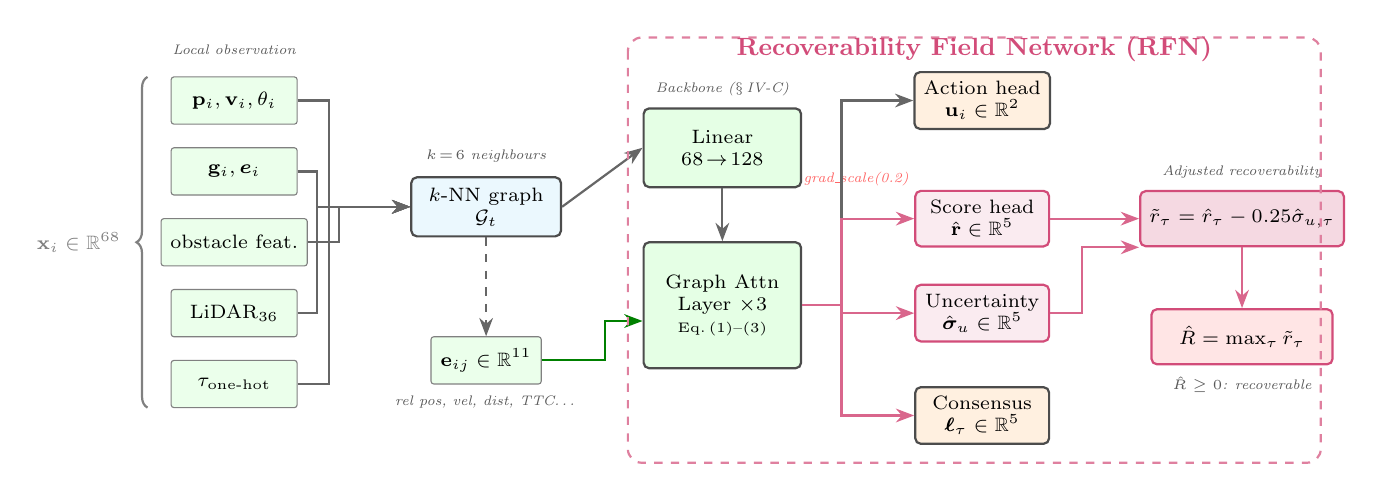
\begin{tikzpicture}[
    >=Stealth,
    block/.style={
        rectangle, draw=black!70, fill=blue!6,
        minimum height=0.75cm, minimum width=1.9cm,
        font=\scriptsize, align=center, rounded corners=2pt,
        thick
    },
    feat/.style={
        rectangle, draw=black!50, fill=green!8,
        minimum height=0.6cm, minimum width=1.6cm,
        font=\scriptsize, align=center, rounded corners=1pt,
    },
    head/.style={
        rectangle, draw=black!70, fill=orange!12,
        minimum height=0.7cm, minimum width=1.7cm,
        font=\scriptsize, align=center, rounded corners=2pt,
        thick
    },
    score/.style={
        rectangle, draw=purple!70, fill=purple!8,
        minimum height=0.7cm, minimum width=1.7cm,
        font=\scriptsize, align=center, rounded corners=2pt,
        thick
    },
    arr/.style={->, thick, black!60},
    garr/.style={->, thick, green!50!black},
    parr/.style={->, thick, purple!60},
    note/.style={font=\tiny\itshape, text=gray!70!black},
]

% ── Column 1: Observation ──
\node[feat] (pos)   at (0, 0.0) {$\bfp_i, \bfv_i, \theta_i$};
\node[feat] (goal)  at (0,-0.9) {$\mathbf{g}_i, \bm{e}_i$};
\node[feat] (obs)   at (0,-1.8) {obstacle feat.};
\node[feat] (lidar) at (0,-2.7) {LiDAR$_{36}$};
\node[feat] (topo)  at (0,-3.6) {$\tau_{\text{one-hot}}$};

\node[note, above=0.15cm of pos] {Local observation};

% ── Brace ──
\draw[decorate, decoration={brace, amplitude=4pt, mirror},
      thick, black!50]
    (-1.1, 0.3) -- (-1.1,-3.9)
    node[midway, left=6pt, font=\scriptsize, align=right]
    {$\mathbf{x}_i \in \mathbb{R}^{68}$};

% ── Column 2: Graph construction ──
\node[block, fill=cyan!8] (knn) at (3.2,-1.35)
    {$k$-NN graph\\$\mathcal{G}_t$};
\node[note, above=0.05cm of knn] {$k\!=\!6$ neighbours};

\draw[arr] (pos.east)   -- ++(0.4,0) |- (knn.west);
\draw[arr] (goal.east)  -- ++(0.25,0) |- (knn.west);
\draw[arr] (obs.east)   -- ++(0.4,0) |- (knn.west);
\draw[arr] (lidar.east) -- ++(0.25,0) |- (knn.west);
\draw[arr] (topo.east)  -- ++(0.4,0) |- (knn.west);

% ── Edge features label ──
\node[feat, minimum width=1.4cm] (efeat) at (3.2,-3.3)
    {$\mathbf{e}_{ij} \in \mathbb{R}^{11}$};
\node[note, below=0.02cm of efeat]
    {rel pos, vel, dist, TTC\ldots};
\draw[arr, dashed] (knn.south) -- (efeat.north);

% ── Column 3: Backbone ──
\node[block, fill=green!10, minimum height=1.0cm,
      minimum width=2.0cm]
    (enc) at (6.2,-0.6) {Linear\\$68 \!\to\! 128$};
\node[block, fill=green!10, minimum height=1.6cm,
      minimum width=2.0cm]
    (gat) at (6.2,-2.6) {Graph Attn\\Layer $\times 3$\\{\tiny Eq.\,(1)--(3)}};

\draw[arr] (knn.east) -- (enc.west);
\draw[arr] (enc.south) -- (gat.north);
\draw[garr] (efeat.east) -- ++(0.8,0) |- ([yshift=-0.2cm]gat.west);

\node[note] at (6.2, 0.15) {Backbone ($\S$\,IV-C)};

% ── Column 4: Heads (branch) ──
% Action
\node[head] (act) at (9.5, 0.0)
    {Action head\\$\bfu_i \in \mathbb{R}^2$};
% Score
\node[score] (rscore) at (9.5,-1.5)
    {Score head\\$\hat{\mathbf{r}} \in \mathbb{R}^5$};
% Uncertainty
\node[score] (unc) at (9.5,-2.7)
    {Uncertainty\\$\hat{\bm{\sigma}}_u \in \mathbb{R}^5$};
% Consensus
\node[head] (cons) at (9.5,-4.0)
    {Consensus\\$\bm{\ell}_\tau \in \mathbb{R}^5$};

% grad scale annotation
\node[note] at (7.9, -1.0) {\textcolor{red!60}{grad\_scale(0.2)}};

\draw[arr] (gat.east) -- ++(0.5,0) |- (act.west);
\draw[parr] (gat.east) -- ++(0.5,0) |- (rscore.west);
\draw[parr] (gat.east) -- ++(0.5,0) |- (unc.west);
\draw[parr] (gat.east) -- ++(0.5,0) |- (cons.west);

% ── Column 5: RFN output ──
\node[score, fill=purple!15, minimum width=2.3cm]
    (rfn_out) at (12.8,-1.5)
    {$\tilde{r}_\tau = \hat{r}_\tau - 0.25\hat{\sigma}_{u,\tau}$};
\node[note, above=0.02cm of rfn_out]
    {Adjusted recoverability};
\draw[parr] (rscore.east) -- (rfn_out.west);
\draw[parr] (unc.east) -- ++(0.4,0) |- (rfn_out.south west);

% RFN margin
\node[score, fill=red!10, minimum width=2.3cm]
    (margin) at (12.8,-3.0)
    {$\hat{R} = \max_\tau \tilde{r}_\tau$};
\draw[parr] (rfn_out.south) -- (margin.north);

\node[note, below=0.02cm of margin]
    {$\hat{R} \ge 0$: recoverable};

% ── Dashed box: RFN ──
\draw[thick, dashed, purple!50, rounded corners=5pt]
    (5.0, 0.8) rectangle (13.8, -4.6);
\node[font=\small\bfseries, text=purple!70]
    at (9.4, 0.65) {Recoverability Field Network (RFN)};

\end{tikzpicture}

\caption{Recoverability Field Network (RFN). Local node and edge
features are encoded by a three-layer graph-attention backbone and
decoded into action, recoverability, uncertainty, and topology outputs.
The adjusted score map $\tilde{r}_\tau$ is used by the topology selector
and by the shield trigger.}
\label{fig:rfn}
\end{figure*}

\subsection{Counterfactual Topology Selection}
\label{sec:selector}

At inference, RVT-Swarm evaluates all candidate topologies using a
combination of recoverability score, topology prior, contextual bonuses,
uncertainty penalty, and switching cost:
\begin{equation}
C_\tau = 0.62\,\tilde{r}_\tau
       + 0.22\,\pi_\tau
       + b_\tau^{\text{ctx}}
       - 0.08\,\sigma_\tau
       - \psi_\tau^{\text{switch}}.
\label{eq:selector}
\end{equation}
The context term favors, for example, \textsc{line} or
\textsc{compress} in bottlenecks and \textsc{recover} once the
bottleneck clears. The switch penalty discourages excessive topology
changes, especially disruptive split actions. A new topology is adopted
only if it exceeds the previous topology by a hysteresis margin, and a
cooldown period suppresses immediate repeated switching. The online
selection-and-shield loop is summarized in \Cref{alg:selector}.

\removelatexerror
\begin{algorithm}[H]
\caption{Counterfactual Topology Selection with Projection Shield}
\label{alg:selector}
\SetAlgoLined
\KwIn{Observation $o_t$, topology logits $\bm{\ell}$, adjusted scores
$\tilde{\mathbf{r}}$, uncertainty $\bm{\sigma}$, previous topology
$\tau_{\mathrm{prev}}$, nominal action $\bfu$}
\KwOut{Selected topology $\tau^\star$, shielded action $\bfu^{\mathrm{safe}}$}
\If{$t - t_{\text{last-switch}} < T_{\text{cool}}$}{
    $\tau^\star \leftarrow \tau_{\mathrm{prev}}$\;
}
\Else{
    Compute prior $\bm{\pi} = \mathrm{softmax}(\bm{\ell}/T)$\;
    Compute contextual bonuses $b_\tau^{\mathrm{ctx}}$\;
    Compute switching penalties $\psi_\tau^{\mathrm{switch}}$\;
    Compute $C_\tau$ using~\eqref{eq:selector}\;
    $\tau' \leftarrow \argmax_{\tau \in \cT} C_\tau$\;
    \eIf{$C_{\tau'} < C_{\tau_{\mathrm{prev}}} + \eta$}{
        $\tau^\star \leftarrow \tau_{\mathrm{prev}}$\;
    }{
        $\tau^\star \leftarrow \tau'$\;
    }
}
\tcp{Risk-triggered projection shield}
$\rho \leftarrow \mathrm{CollisionRisk}(o_t)$\;
\If{$\max_{\tau \in \cT}\tilde{r}_\tau < 0$}{
    $\rho \leftarrow \max(\rho, \rho_{\mathrm{crisis}})$\;
}
\If{$\rho \ge \rho_{\mathrm{th}}$}{
    Build pairwise robot-robot and robot-obstacle half-planes\;
    Project $\bfu$ onto the feasible intersection and acceleration ball\;
    Blend projected and nominal actions to obtain $\bfu^{\mathrm{safe}}$\;
}
\Else{
    $\bfu^{\mathrm{safe}} \leftarrow \bfu$\;
}
\Return{$\tau^\star, \bfu^{\mathrm{safe}}$}
\end{algorithm}

\subsection{Progress-Preserving Projection Shield}
\label{sec:shield}

The shield activates only when collision risk is high or when all
candidate topologies have negative recoverability. Pairwise robot-robot
and robot-obstacle constraints are converted into half-plane
constraints in action space using a CBF-inspired linearization. For
robot $i$, we use the barrier
\begin{equation}
h_{ij} = \|\bfp_i - \bfp_j\|^2 - d_{\text{safe}}^2
\label{eq:barrier}
\end{equation}
and enforce
\begin{equation}
\nabla h_{ij}^{\top}\bfu_i \ge
-\alpha h_{ij} - 2(\bfp_i - \bfp_j)^\top(\bfv_i - \bfv_j).
\label{eq:cbf_constraint}
\end{equation}
Rather than solving a full external QP, we iteratively project a
progress-biased target action onto the intersection of these half-planes
and the acceleration ball. The final shielded action is softly blended
with the learned action, which reduces overreaction near the risk
threshold.

\section{Training}
\label{sec:training}

\subsection{Data Generation}
Training data are generated from a common heuristic expert controller in
the shared simulator. For each sampled state, we run short-horizon
counterfactual rollouts for every topology in $\cT$ using the same
expert controller, producing:
\begin{itemize}
    \item a per-topology score vector;
    \item a best-topology label;
    \item a scalar recoverability margin derived from the score gap and
    the best score.
\end{itemize}
The current release uses 500 episodes spanning four scenarios
(\emph{open field}, \emph{cluttered}, \emph{narrow passage},
\emph{dynamic obstacles}) and team sizes
$N \in \{4,8,12,16\}$. Hard-negative mining augments difficult
bottleneck states with perturbed actions.

\subsection{Loss and Optimization}
For RVT-Swarm, the training loss is
\begin{multline}
\mathcal{L} =
\lambda_a \mathcal{L}_{\text{act}}
 + \lambda_r \mathcal{L}_{\text{rec}}
 + \lambda_\tau\bigl(
   \mathcal{L}_{\text{topo}}
 + 0.8\,\mathcal{L}_{\text{score}}
 + 0.45\,\mathcal{L}_{\text{rank}}
 \bigr) \\
 + \lambda_x \mathcal{L}_{\text{aux}}
 + \mathcal{L}_{\text{unc}},
\label{eq:loss}
\end{multline}
where the terms correspond respectively to action regression,
recoverability regression, topology classification, score-map
regression, pairwise topology ranking, auxiliary environment-state
prediction, and uncertainty regularization. The current hyperparameters
are $\lambda_a=5.0$, $\lambda_r=0.02$, $\lambda_\tau=0.01$, and
$\lambda_x=0.004$.

Auxiliary losses are linearly ramped in over a 50-epoch warmup for
RVT-Swarm. The three learned methods are trained with AdamW
($3\times10^{-4}$ learning rate, $10^{-5}$ weight decay, batch size
32). Best-checkpoint selection is based on periodic rollout validation:
after warmup, every five epochs we evaluate a small validation set over
\emph{narrow passage} and \emph{dynamic obstacles} for team sizes 8 and
16, and select checkpoints using a score that combines success,
collision-free execution, formation quality, deadlock, stall, and
collapse.

\section{Experiments}
\label{sec:experiments}

\subsection{Experimental Protocol}
The benchmark uses a common 2D simulator with workspace
$12\times12$\,m, time step $\Delta t = 0.15$\,s, robot radius
0.18\,m, obstacle radius 0.35\,m, speed limit 0.9\,m/s, acceleration
limit 0.6\,m/s$^2$, and a 36-ray LiDAR with 3\,m range. Main evaluation
uses 25 episodes per setting over 4 scenarios and 4 team sizes, for
400 episodes per method. Episodes are matched across methods by shared
seeds.

\paragraph{Implementation scope.}
This benchmark is intentionally a \emph{common-simulator prototype}.
The non-learned baselines (\textsc{adaptive\_formation},
\textsc{cbf\_qp\_like}, \textsc{orca\_like}, and
\textsc{centralized\_mpc}) are internal normalized baselines rather than
exact package-level reproductions. The current paper reports the
single-seed result produced by the released code path; multi-seed
confidence intervals remain future work.

\subsection{Compared Methods}
\textbf{GNN-Only} uses the shared graph backbone with only an action
head. \textbf{InstantCert} adds a scalar recoverability-style head but
no topology adaptation. \textbf{RVT-Swarm} is the full model.
Historical baselines include a heuristic adaptive-formation controller,
a CBF-QP-like reactive filter, ORCA-like avoidance, and a centralized
MPC-inspired proxy.

\subsection{Main Results}
\label{sec:main_results}

\begin{table*}[!t]
\centering
\caption{Main benchmark results averaged over all scenarios and team
sizes. Numbers are from the current single-seed prototype run.}
\label{tab:main_results}
\scriptsize
\begin{tabular}{lccccccccc}
\toprule
\textbf{Method}
& \textbf{Success}$\uparrow$
& \textbf{Goal}$\uparrow$
& \textbf{Coll-Free}$\uparrow$
& \textbf{Form OK}$\uparrow$
& \textbf{Form RMS}$\downarrow$
& \textbf{Stall}$\downarrow$
& \textbf{Deadlock}$\downarrow$
& \textbf{Collapse}$\downarrow$
& \textbf{ms/step}$\downarrow$ \\
\midrule
ORCA-like          & 0.000 & \textbf{0.932} & 0.625 & 0.000 & 2.930 & \textbf{0.000} & \textbf{0.000} & \textbf{0.020} & \textbf{1.0} \\
Adaptive Formation & 0.288 & 0.785 & 0.565 & 0.348 & 0.952 & 0.026 & 0.075 & 0.120 & \textbf{1.0} \\
CBF-QP-like        & 0.188 & 0.728 & \textbf{0.718} & 0.210 & 0.842 & 0.028 & 0.093 & 0.095 & \textbf{1.0} \\
Centralized MPC    & 0.315 & 0.770 & 0.630 & 0.340 & 0.951 & 0.025 & 0.108 & 0.160 & \textbf{1.0} \\
\midrule
GNN-Only           & 0.390 & 0.788 & 0.645 & 0.428 & 0.760 & 0.027 & 0.085 & 0.125 & \textbf{1.0} \\
InstantCert        & 0.413 & 0.772 & 0.655 & 0.453 & \textbf{0.733} & 0.031 & 0.098 & 0.135 & \textbf{1.0} \\
\textbf{RVT-Swarm} & \textbf{0.435} & 0.760 & 0.660 & \textbf{0.478} & 0.764 & \textbf{0.023} & \textbf{0.068} & \textbf{0.113} & 1.6 \\
\bottomrule
\end{tabular}
\end{table*}

Three points stand out from \Cref{tab:main_results}.
First, RVT-Swarm achieves the highest composite success among all
methods. The margin over InstantCert is modest in absolute terms
($+2.25$ percentage points) but consistent with the intended role of
recoverability-aware topology adaptation. Second, RVT-Swarm produces the
highest formation-success rate among learned methods
(\textbf{47.75\%} \texttt{form\_ok}) and the lowest deadlock rate among
methods that still preserve formation. Third, the table exposes the
trade-offs of the baselines: ORCA-like motion reaches the goal often but
abandons formation entirely, while CBF-QP-like control maximizes
collision-free execution at the cost of formation completion.

\subsection{Ablation Results}
\label{sec:ablation}

\begin{table}[H]
\centering
\caption{Ablation results for RVT-Swarm. The current prototype ablation
study is intentionally reported \emph{as is}: the full model is not
uniformly best on every metric.}
\label{tab:ablation}
\scriptsize
\resizebox{\columnwidth}{!}{%
\begin{tabular}{lcccccc}
\toprule
\textbf{Variant}
& \textbf{Success}$\uparrow$
& \textbf{Coll-Free}$\uparrow$
& \textbf{Form OK}$\uparrow$
& \textbf{Deadlock}$\downarrow$
& \textbf{Collapse}$\downarrow$
& \textbf{Topo Sw.}$\downarrow$ \\
\midrule
Full                & 0.398 & \textbf{0.663} & 0.425 & 0.060 & 0.118 & 0.262 \\
$-$ Recoverability  & \textbf{0.405} & 0.640 & 0.438 & 0.090 & 0.140 & 0.455 \\
$-$ Counterfactual  & \textbf{0.405} & 0.638 & 0.450 & \textbf{0.045} & \textbf{0.095} & 0.820 \\
$-$ Progress shield & \textbf{0.405} & 0.630 & \textbf{0.458} & 0.065 & 0.100 & 0.333 \\
$-$ Topology        & 0.400 & 0.625 & 0.438 & 0.095 & 0.133 & \textbf{0.000} \\
Fixed formation     & 0.385 & 0.655 & 0.415 & 0.080 & 0.140 & \textbf{0.000} \\
\bottomrule
\end{tabular}
\vspace{1mm}
}
\end{table}

The ablation study is the most important reason to keep the current
paper honest. The full model is \emph{best on the main benchmark}, but
it is not best on every ablation metric. Removing recoverability,
counterfactual selection, or the progress shield slightly improves
success in this particular ablation sweep, whereas the full model
achieves the best collision-free rate. Meanwhile, removing
counterfactual scoring produces very high topology switching
($0.82$), suggesting that the counterfactual selector is stabilizing the
policy even when its effect on success is not yet dominant. Taken
together, these results support a nuanced conclusion: the RVT ingredients
matter, but their present coupling is still imperfect.

\subsection{Interpretation}
The results suggest that RVT-Swarm wins primarily by balancing
formation completion against liveness failure modes. Compared with
InstantCert and GNN-Only, it reduces deadlock and collapse while keeping
collision-free performance competitive. At the same time, the ablation
table shows that the recoverability proxy and the end-task objective are
not yet perfectly aligned. This is consistent with the codebase design:
recoverability labels are short-horizon counterfactual surrogates rather
than exact viability certificates, and the selector/shield operates with
simple contextual bonuses rather than a fully optimized planner.

\section{Limitations and Future Work}
\label{sec:limitations}

This work should be read as a research prototype with promising
algorithmic structure, not as a finished benchmark artifact.
The main limitations are:
\begin{itemize}
    \item \textbf{Short-horizon recoverability surrogate.}
    Recoverability labels are derived from a heuristic expert over a
    finite horizon rather than from a globally optimal planner or a
    formally certified reachability computation.

    \item \textbf{Prototype baselines.}
    The historical baselines are normalized in-house implementations in
    a common simulator, not exact reproductions of external packages.

    \item \textbf{Single-seed reporting.}
    The current paper reports one full prototype sweep. A submission
    intended for a top-tier venue should include multi-seed confidence
    intervals, statistical testing, and a more mature baseline suite.

    \item \textbf{Simplified shield and dynamics.}
    The shield uses iterative half-plane projection, and the environment
    is 2D with simplified kinematics. Extensions to nonholonomic and 3D
    platforms remain open.
\end{itemize}

The clearest next steps are to (i) align checkpointing and training
losses more directly with rollout success, (ii) strengthen the
recoverability label generation with better local planning or longer
horizons, and (iii) evaluate the method over multiple seeds and richer
baseline reproductions.

\section{Conclusion}
\label{sec:conclusion}

We presented RVT-Swarm, a decentralized graph-based controller that
combines continuous control, discrete topology adaptation, and a learned
recoverability score map for swarm formation control in constrained
environments. The current implementation demonstrates that this design
can outperform simpler learned baselines on the main benchmark and can
reduce deadlock and irreversible collapse, while also revealing through
ablation that the recoverability-selector-shield coupling still leaves
headroom for improvement.

\bibliographystyle{IEEEtran}
\bibliography{references}

\appendix

\section*{Appendix: Current Hyperparameters}
\label{app:hyperparams}

\begin{table}[H]
\centering
\caption{Current hyperparameter settings in the released prototype.}
\label{tab:hyperparams}
\scriptsize
\begin{tabular}{ll}
\toprule
\textbf{Parameter} & \textbf{Value} \\
\midrule
\multicolumn{2}{l}{\emph{Environment}} \\
Workspace & $12.0 \times 12.0$\,m \\
$\Delta t$ & 0.15\,s \\
$v_{\max}$ / $u_{\max}$ & 0.9 / 0.6 \\
Robot / obstacle radius & 0.18 / 0.35 \\
LiDAR rays / range / FOV & 36 / 3.0\,m / 270$^\circ$ \\
Team sizes & \{4, 8, 12, 16\} \\
Scenarios & open, cluttered, narrow, dynamic \\
\midrule
\multicolumn{2}{l}{\emph{Model}} \\
Node feature dim / edge dim & 68 / 11 \\
Hidden dim / message passes & 128 / 3 \\
Graph neighborhood $k$ & 6 \\
Aux gradient scale & 0.2 \\
\midrule
\multicolumn{2}{l}{\emph{Training}} \\
Expert episodes & 500 \\
Batch size & 32 \\
Learning rate / weight decay & $3\times10^{-4}$ / $10^{-5}$ \\
Recoverability horizon $H$ & 14 \\
$\lambda_a / \lambda_r$ & 5.0 / 0.02 \\
$\lambda_\tau / \lambda_x$ & 0.01 / 0.004 \\
RVT warmup epochs & 50 \\
Early stopping patience & 40 \\
RVT max epochs & 300 \\
GNN / InstantCert max epochs & 120 / 120 \\
\midrule
\multicolumn{2}{l}{\emph{Rollout validation}} \\
Enabled & yes \\
Interval & every 5 epochs \\
Scenarios & narrow passage, dynamic obstacles \\
Team sizes & 8, 16 \\
Episodes per setting & 2 \\
\midrule
\multicolumn{2}{l}{\emph{Inference}} \\
Switch hysteresis & 0.08 \\
Topology cooldown & 12 steps \\
Topology temperature & 1.5 \\
Shield risk threshold & 0.85 \\
Max shield blend & 0.06 \\
\midrule
\multicolumn{2}{l}{\emph{Evaluation}} \\
Episodes per setting & 25 \\
\bottomrule
\end{tabular}
\end{table}

\end{document}
